% ****** Start of file apssamp.tex ******
%
%   This file is part of the APS files in the REVTeX 4.1 distribution.
%   Version 4.1r of REVTeX, August 2010
%
%   Copyright (c) 2009, 2010 The American Physical Society.
%
%   See the REVTeX 4 README file for restrictions and more information.
%
% TeX'ing this file requires that you have AMS-LaTeX 2.0 installed
% as well as the rest of the prerequisites for REVTeX 4.1
%
% See the REVTeX 4 README file
% It also requires running BibTeX. The commands are as follows:
%
%  1)  latex apssamp.tex
%  2)  bibtex apssamp
%  3)  latex apssamp.tex
%  4)  latex apssamp.tex
%
\documentclass[%
 reprint,
 %twocolumn,
%superscriptaddress,
%groupedaddress,
%unsortedaddress,
%runinaddress,
%frontmatterverbose, 
%preprint,
%showpacs,preprintnumbers,
%nofootinbib,
%nobibnotes,
%bibnotes,
 amsmath,amssymb,
 aps,
%pra,
%prb,
%rmp,
%prstab,
%prstper,
floatfix,
]{revtex4-1}

\usepackage{graphicx}% Include figure files
\usepackage{dcolumn}% Align table columns on decimal point
\usepackage{bm}% bold math
%\usepackage{hyperref}% add hypertext capabilities
%\usepackage[mathlines]{lineno}% Enable numbering of text and display math
%\linenumbers\relax % Commence numbering lines

%\usepackage[showframe,%Uncomment any one of the following lines to test 
%scale=0.7, marginratio={1:1, 2:3}, ignoreall,% default settings
%text={7in,10in},centering,
%margin=1.5in,
%total={6.5in,8.75in}, top=1.2in, left=0.9in, includefoot,
%height=10in,a5paper,hmargin={3cm,0.8in},
%]{geometry}

\newcommand{\dd}{\mathrm{d}}

%%%%%%%%%%%%%%%%%
\usepackage[usenames,dvipsnames]{xcolor}
%%%%%%%%%%%%%%%%%

\begin{document}

\preprint{APS/123-QED}

\title{A simple mechanism for higher-order correlations\\ in integrate-and-fire neurons}% Force line breaks with \\

\author{David A. Leen}
\email{dleen@washington.edu}

%Lines break automatically or can be forced with \\
 
\author{Eric Shea-Brown}%
\email{etsb@washington.edu}
\affiliation{%
Department of Applied Mathematics, University of Washington.
}

\date{\today}% It is always \today, today,
             %  but any date may be explicitly specified

\begin{abstract}
Here we show that a population of exponential integrate-and-fire neurons receiving common input cannot be well described by a pairwise maximum entropy model. A tractable reduction of the EIF model, the linear filter, also gives rise to higher-order correlations. 
\end{abstract}

\pacs{87.19.lj}% PACS, the Physics and Astronomy
                             % Classification Scheme.
%\keywords{Suggested keywords}%Use showkeys class option if keyword
                              %display desired
\maketitle

%\tableofcontents
%%%%%%%%%%%%%%%%%%%
\section{\label{sec:intro}Introduction}%
%%%%%%%%%%%%%%%%%%%
Recent work by Macke et.~al~\cite{Macke:2011gw} shows that common input gives rise to higher-order correlations in the Dichotomized Gaussian neuron model. Motivated by this finding we investigate whether the same holds true when one considers biologically plausible neuron models such as integrate-and-fire neurons. Prove that common input to EIF model, a biologically plausible model of a neuron, cannot be described by the pairwise maximum entropy (Ising) model i.e.~a model only taking into account first and second moments. That common input into the EIF is an easy way of realizing higher-order correlations.

Propose tractable reduction of EIF: linear model. This linear model can also capture higher-order correlations. So we can suggest linear point process models for higher-order correlations. Demonstrate effectiveness versus PME model.

Can we show that this linear model helps us understand why the EIF and DG models are so similar?

Can we show some study in the opposite sense: that max ent works for larger populations. Ganmor?

Values of correlation coefficients in literature?

 \colorbox{BrickRed}{\color{White}{Incomplete.}}

%%%%%%%%%%%%%%%%%%%
\section{\label{sec:models}Models}   %
%%%%%%%%%%%%%%%%%%%
%%%%
% EIF %
%%%%
\paragraph*{The exponential integrate-and-fire model.}
The model consists of a homogeneous population of $N$ exponential integrate-and-fire (EIF) neurons, receiving common white noise inputs $\xi_c(t)$ and independent white noise inputs $\xi_i(t)$, whose membrane voltage evolves according to the equation: 
\begin{align}
\label{eifsde}
\tau_m V_i^\prime &= -V_i +\psi(V_i)+I(t),\\
I(t) &= \gamma+\sqrt{\sigma^2\tau_m}\big[\sqrt{1-\lambda}\xi_i(t)+\sqrt{\lambda}\xi_c(t)\big] \nonumber,
\end{align}
where: $\psi(V_i) =\Delta_T \exp{\left((V_i - V_S)/\Delta_T\right)}$ for the EIF neuron. Here, $\tau_m$ is the membrane time constant, $\Delta_T$ controls the slope of the action potential initiation. We use the usual convention of declaring a spike whenever the voltage reaches a certain threshold $V_T$, which we have set at $20$mV. The EIF neuron has an additional ``soft'' threshold, $V_S$ beyond which the voltage diverges to infinity. We set this value as $-53$mV. After a spike the voltage is reset to the rest potential $V_R$, set at $-60$mV, and is held there for the duration of the refractory period $\tau_{\text{ref}}$ of $3$ms.

The input current has a constant (DC) component $\gamma$, considered the effective rest potential in the absence of noise, and a stochastic noise component with amplitude $\sigma$. The input is modeled by a correlated Gaussian with mean $\gamma$, and covariance $\lambda$. The output spike trains have a mean $\mu$ and covariance $\alpha$. For comparisons across models, the mean firing rate $\mu$ describes the mean number of spikes in each bin. Following~\cite{Macke:2011gw} we define the pairwise correlation coefficient $\rho = \alpha/\mu(1-\mu)$.

The spikes are binned into bins of temporal resolution $T_\text{bin}$, which we choose to be $10$ms. On rare occasions multiple spikes from the same neuron can occur in the same bin. These are considered as a single spike. For a mean firing rate of $\mu=0.1$ and correlation $\rho=0.1$,  multiply binned spikes represent less than $0.4\%$ of all spiking events in our numerical simulations.

We tune our model so that when the DC component of the input $\gamma$ is set, in the absence of common input i.e.~$\lambda = 0$, as $\gamma = -60$mV (rest potential), the neurons fire at a rate given by $\mu = 0.1$ or equivalently $10$Hz (given that the bin size $\Delta t = 10$ms). This constrains our noise amplitude to be $\sigma = 6.23$mV.
%%%%%%%%%%%%%%%%%%
\begin{figure*}
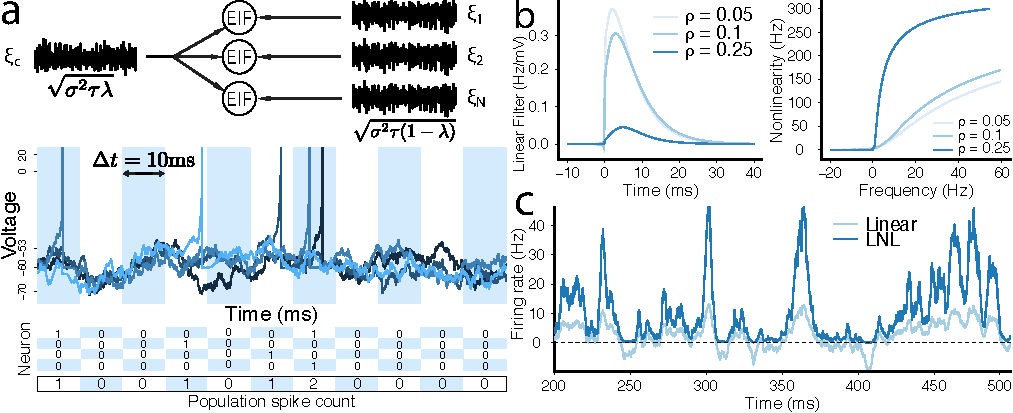
\includegraphics{../R/fig_1/fig_1_final}
\caption{\label{fig:schematic} Schematic of the models: (a) exponential integrate-and-fire neurons receiving common input $\xi_c$ and independent inputs $\xi_i$. The voltages of the neurons evolve according to equation [\ref{eifsde}]. Time is divided into bins of temporal resolution $10$ms. A spike occurs when the voltage reaches a threshold of $20$mV. The voltage is then reset to the resting potential $-60$mV and another spike cannot occur during the refractory period of $3$ms. Spikes recorded from each of the EIF neurons in a bin contribute towards the population spike count. More than one spike occurring from the same neuron within a single bin is treated as a single event. This happens less than $0.4\%$ of the time in our numerical simulations. (b) The linear filter $A(t)$ and static non-linearity for different values of the correlation coefficient $\rho$. The filter receives a noise amplitude of $\sigma\sqrt{1-\lambda}$. The static-nonlinearity receives a noise amplitude of $\sigma$. (c) The static non-linearity applied to the linear estimate of the firing rate, for $\mu = 0.1$, $\rho = 0.1$. The non-linearity increases the firing rate magnitude and rectifies negative firing rates. The firing rate is used to generate spikes, treating the spike output from repeated presentations of the firing rate as coming from a population of uncoupled neurons to arrive at a population spike count such as in (a).}
\end{figure*}
%%%%%%%%%%%%%%%%%
%%%%
% LNL %
%%%%
\paragraph*{The linear-nonlinear model.}
The simplest case a of general linear model is the linear-nonlinear cascade, where the firing rate of a neuron is estimated by convolving a temporal filter with an input signal and then applying a time independent nonlinear function. The neurons are represented as exponential integrate-and-fire spiking neurons receiving a time varying current consisting of two components: a time varying input that is identical in all trials (the common input) and a background noise that is uncorrelated from trial to trial (the independent input). The resulting firing rate can then be interpreted as the firing rate of $N$ uncoupled neurons that all receive an identical input signal as well as background noise that is uncorrelated from neuron to neuron. 

Following the EIF model the noise input is Gaussian with mean $\gamma$, standard deviation $\sigma$ and no temporal correlation. The statistics of the stimulus signal are Gaussian with mean zero and standard deviation $\sqrt{\sigma^2\tau_m\lambda}$.

In the linear limit the firing rate of the spiking neuron is given by $r(t) = r_0 + A*c(t)$, where $A(t)$ is the response function of the neuron in presence of white noise, and $c(t)$ is the common input: $c(t) = \sqrt{\sigma^2 \tau \lambda}~\xi(t)$. The Fourier transform $\hat{A}(\omega)$ can be calculated numerically for the EIF neuron see [Richardson]. The stationary firing rate $r_0$ can be calculated explicitly.

The total input current to the neuron is used to calculate the stationary firing rate $r_0$, and so receives a noise amplitude of $\sigma$. The filter receives a noise amplitude dependent on the input covariance $\lambda$, the noise amplitude is $\sigma \sqrt{1-\lambda}$. \colorbox{BrickRed}{\color{White}{Reason for the filter noise amplitude being $\sigma\sqrt{1-\lambda}$?}}

Using a static non-linearity $F$ the firing rate is approximated as:
\begin{equation}
r(t) = F\left(r_0+A * c(t) \right), ~F(L) = \Phi\left( \gamma + \frac{L}{\Phi^\prime(\gamma)}\right), \nonumber
\end{equation}
see [Ostoijic] for details, $\Phi$ is the transfer function of the neuron which can be calculated numerically see [Richardson] for details.

For an inhomogeneous Poisson process with rate $r(t)$ conditioned on a common input $c(t)$ the probability of a spike occurring in the interval $[t,t+\Delta t]$ is:
\begin{equation}
P(\text{spike}\in\Delta t | c ) = 1 - \exp{\left(-\int_0^{\Delta t} \! r(s+t) \dd s \right)}.
\end{equation}
To generate spikes from this rate $r(t)$ we could implement this process numerically. We can do this calculation without having to do a numerical simulation: conditioned on a common input the neurons are conditionally independent. We define the new variable, the integral of the firing rate over the course of a time bin:
\begin{equation}
\mathcal{S} = \int_0^{\Delta t} \! r(s) \dd s.
\end{equation}
For the linear estimate, when the static-nonlinearity is the identity $F(L) = L$, the variable $\mathcal{S}$ is Gaussian with $\mathbb{E}(\mathcal{S}) = 0$, $\mathbb{E}(\mathcal{S}^2) = \sigma^2 \tau_m \lambda \int_{-\infty}^{\infty} B^2 (\tau) \dd \tau$, where $B(\tau) = \int_0^{\Delta t} A(t-\tau) \dd t$. However when using the non-linearity, the variable $\mathcal{S}$ is no longer Gaussian and its statistics must be evaluated numerically.
In terms of this variable the neurons are conditionally independent and the probability of observing a spike count $k$ is:
\begin{equation}
P_{\text{LF}}(k) = \binom{n}{k} \int_{-\infty}^{~\infty} \phi_{LF}(\mathcal{S}) \big(1-\tilde{L}\big)^{n-k} \tilde{L}^{k} \dd \mathcal{S}
\end{equation}
where $\tilde{L}(\mathcal{S}) = 1-\exp(-\mathcal{S})$, and $\phi_{LF}(\mathcal{S})$ is the probability density function of the integral of the firing rate over a time bin.

Unlike the exponential-IF model by using this theoretical calculation there are no problems with doubly binned spikes. However, numerically simulating this process of generating spikes from the firing rate double counting occurs quite frequently.
 
 %%%%
% DG %
%%%%
\paragraph*{The Dichotomized Gaussian model.}
The Dichotomized Gaussian is a model of a binary neuron receiving correlated Gaussian input with mean $\gamma$ and covariance $\lambda$. The neuron spikes if its input is positive and is silent otherwise. The mean of the input is chosen so that the mean of the output is $\mu$ and similarly $\lambda$ is chosen so that the correlation coefficient is $\rho$.

The correlated Gaussian can be written as: $Z_i = \gamma + \sqrt{1-\lambda} T_i + \sqrt{\lambda} S$ where $T_i$ is the independent input and  $S$ is the common input. The probability of a spike is given by $P(Z_i > 0 | s)$ and again we can define the $L(s)$ function:
\begin{equation}
L(s) = P\left( T_i > \frac{-s-\gamma}{\sqrt{1-\lambda}} \right) = \Phi\left(\frac{s+\gamma}{\sqrt{1-\lambda}}\right)
\end{equation}
The probability of observing a spike count $k$ is the same as equation [eqnum] using $L(s)$ and $\phi_{DG}(s)$ is the probability density function of a one-dimensional Gaussian with mean $0$ and variance $\lambda$.
%%%%%%%%%%
\section{Results}   %
%%%%%%%%%%
%%%%
% EIF %
%%%%
\paragraph*{The EIF model with common input gives rise to higher-order correlations.}
Difficult to say a whole lot here really. Let's try though: correlations in the exponential integrate-and-fire (EIF) model are not well described by a pairwise maximum entropy model. For small populations the PME does a satisfactory job. For populations larger than about $30$ neurons the PME fails to capture the shape of the distribution, resembling instead a population of independent neurons.
%%%%%%%%%%%%%%
\begin{figure}[h]
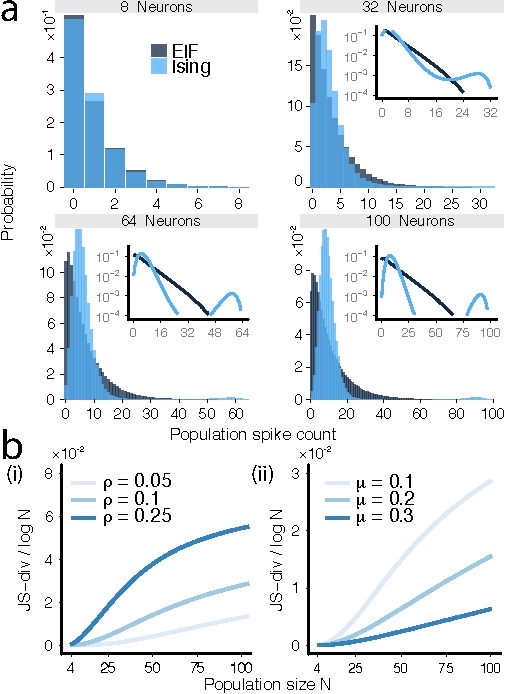
\includegraphics{../R/fig_2/fig_2a_test.pdf}
\caption{\label{fig:eifising}Correlations in the exponential integrate-and-fire (EIF) model are not well described by a pairwise maximum entropy model. (a) A comparison between the population spike-count distributions for the EIF model and it's second-order approximation for $8, 32, 64, \text{and } 100$ neurons for $\mu = 0.1$ and $\rho = 0.1$. The distributions are similar for smaller populations and different for large populations. Inset: the same distributions on a log-linear scale. (b) The Jensen-Shannon (JS) divergence between the EIF and the pairwise maximum entropy (PME) model normalized by the population size, (i) for a constant value of $\mu = 0.1$ and different values of $\rho$, and (ii) for constant value of $\rho = 0.1$ and different values of $\mu$ as the population size increases. The JS-divergence grows with increasing correlation $\rho$ and decreasing mean firing rate $\mu$.}
\end{figure}
%%%%%%%%%%%%%%

Talk about the Jensen-Shannon divergence. Why choose this over the Kullback-Leibler divergence? Choosing JS div allows us to compare between models. The JS div is symmetric and the square root makes it a metric. It can be written in terms of entropies. It is the entropy of the mixture minus one half of the individual entropies. Entropy scales as $\log{N}$ of the population size, this is the upper bound -- which is obtained by the uniform distribution. We have normalized our plots by this to remove the effect of the entropy growing with population size to isolate the effect of higher-order correlations.

We find that JS-div grows with increasing correlation coefficient for a constant mean firing rate $\mu = 0.1$. We also find that the JS-div grows for decreasing mean firing rate at fixed correlation value $\rho = 0.1$. Can we say something about the growth with population size? More than linear?

A change in correlation from $\rho = 0$ to $\rho = 0.2$ causes a massive change for the EIF model but has only a small impact on the PME model.

The effect of the membrane time constant, refractory period, other EIF neuron parameters etc.~ only has the effect of limiting the possible values of the mean firing rate $\mu$. \colorbox{BrickRed}{\color{White}{Incomplete.}}

%%%%%%%%%%%
% LNL CASCADE    %
%%%%%%%%%%%
\paragraph*{The linear-nonlinear cascade model is a tractable reduction of the EIF neuron and provides a simple mechanism for higher-order correlations.}
The linear-nonlinear cascade model provides an effective approximation to the EIF model across a range of population sizes. It offers a vast improvement over the PME model. It has its basis in biological plausibility. It is analytic for the linear estimate, and semi-analytic for the nonlinear version. 
%%%%%%%%%%%%%%
\begin{figure}[h]
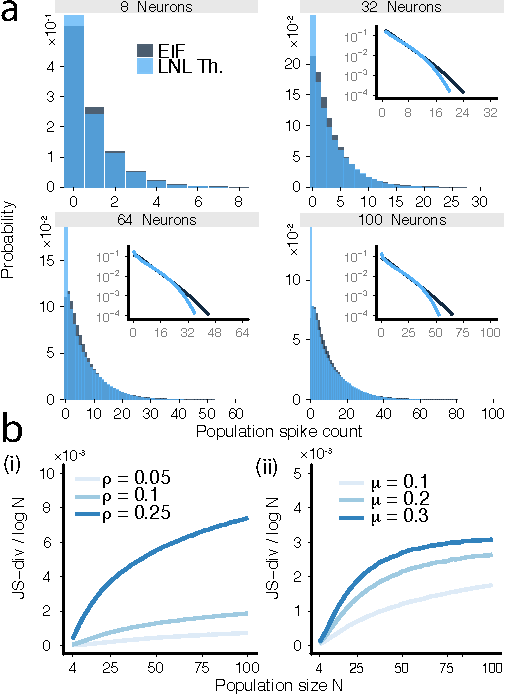
\includegraphics{../R/fig_3/fig_3a_test.pdf}
\caption{\label{fig:eiffilter} The linear-nonlinear cascade gives a good approximation of the EIF population distributions. (a) A comparison between the population spike-count distributions for the EIF model and the linear-nonlinear cascade approximation for $8, 32, 64, \text{and } 100$ neurons for $\mu = 0.1$ and $\rho = 0.1$. The LNL model greatly overestimates the zero population spike count probabilities. One reason is that there is no refractory period. The LNL model underestimates the tails of the probability distributions. This is because of the double counting, when truncating spikes in a bin the larger spike counts are penalized to a greater extent. Inset: the same distributions on a log-linear scale. (b) JS-divergence, order of magnitude smaller than PME, possibly converges to some limit? The order of the mean firing rates is reversed when compared to the PME because the LNL cascade gives a better approximation at higher firing rates $\mu$, less problems with negative firing rates...}
\end{figure}
%%%%%%%%%%%%%%%

The LNL model has obvious problems -- the worst offender being the overestimation of the zero spike states $P(0)$, in the $N=100$ case it overestimates by almost $100\%$. Why is this the case? I don't have a good answer other than looking at the $L(s)$ function. Overestimating zero spike probability does not occur for $\rho = 0.05$. This probably gives us a clue. Possible answer: negative firing rates are rectified to rates slightly greater than zero. This leads to large periods of almost zero firing rates. Fraction of linear estimate of firing rate is negative $20\%$ of the time for $\rho = 0.05$, and $30\%$ of the time for $\rho=0.1$.

The LNL also underestimates the tail of the distribution. This also needs an explanation. Maybe the higher frequency estimate of the firing rate is too low? Maybe it's not at a high enough firing rate for long enough? There is a way to fix this in the numerical simulations but not in the theory. In the numerical simulations you can allow extra spikes in a bin to contribute to the total. Maybe it's because the nonlinearity saturates, there is a maximum allowable firing rate.

The JS-div between the EIF model and the linear-nonlinear model is an order of magnitude better estimate than the PME model. Does it look like it's converging? Can we do $N=200$? The order of the mean firing rate order is reversed when compared to the EIF model. \colorbox{BrickRed}{\color{White}{Incomplete.}}

%%%%
% DG %
%%%%
%\paragraph*{The Dichotomized Gaussian model provides an excellent approximation to the EIF model.}
%Lorem ipsum dolor sit amet, consectetur adipisicing elit, sed do eiusmod tempor incididunt ut labore et dolore magna aliqua. \colorbox{BrickRed}{\color{White}{Incomplete.}}
%%%%%%%%%%%%%%
%%%%%%%%%%%%%%%


%%%%%%%%%%%%%%%%
% Comparison: LNL and DG   %
%%%%%%%%%%%%%%%%
\paragraph*{The linear-nonlinear model approximates the Dichotomized Gaussian model.}
\begin{figure*}
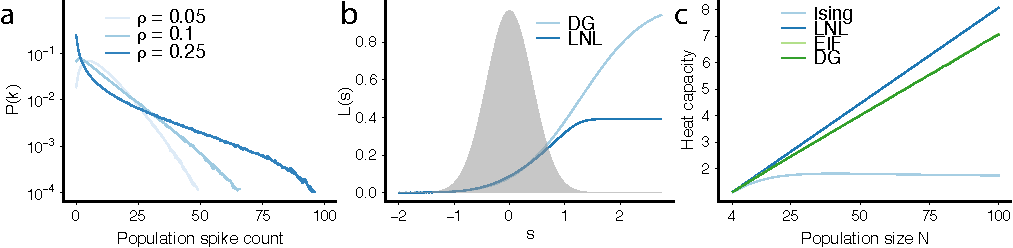
\includegraphics{../R/fig_4/fig_4.pdf}
\caption{\label{fig:lnldgcomp} (a) The Dichotomized Gaussian (DG) model gives an excellent description of the exponential integrate-and-fire (EIF) population spike count probability distributions across a range of correlation coefficient values. The two models are plotted on top of one another and appear as a single curve for each value of $\rho$. (b) Comparing the $L(s)$ function for the DG and the $\tilde{L}(s)$ function for the EIF (after transforming from the EIF probability density function for the variable $\mathcal{S}$ to the DG variable $s$. The functions agree to an extent over the pdf $\phi_DG$ of the DG model. The DG function $L(s)$ tends to $0$ for negative values of $s$ where the LNL function $\tilde{L}(s)$ tends to a finite non-zero value. This agrees with the probability distributions in the previous model where the LNL cascade is less accurate at estimating the $0$-population spike count and large population spike count probabilities. (c) The heat capacity increases linearly for the LNL-cascade, the EIF and the DG. For the case of the LNL cascade the heat capacity increases at a slightly greater rate than the EIF/DG which overlap. The Ising model saturates for a population of approximately $N=20$ neurons.}
\end{figure*}
To compare the linear-nonlinear model to the Dichotomized Gaussian model we look at the probability distributions $P_{\text{LNL}}$ and $P_{\text{DG}}$. To make the comparison we must transform from the probability density function of the linear-nonlinear model $\phi_{LF}$ to the Gaussian pdf $\phi_{DG}$ using the change of variable:
\begin{equation}
\mathcal{S} = f(s),\quad\text{where}\quad f^\prime(s) = \frac{\phi_{DG}(s)}{\phi_{LF}\big(f(s)\big)}.
\end{equation}
This means that:
\begin{equation}
P_{\text{LF}}(k) = \binom{n}{k}\!\!\int_{-\infty}^{~\infty} \phi_{\text{DG}}(s) \big(1-\tilde{L}(f(s))\big)^{n-k} \tilde{L}(f(s))^{k} \dd s
\end{equation}
and to compare to the Dichotomized Gaussian model we only need to compare the $L(s)$ functions. \colorbox{BrickRed}{\color{White}{Incomplete.}}


%%%%%%%%%%%%
\section{Conclusion}   %
%%%%%%%%%%%%
Lorem ipsum dolor sit amet, consectetur adipisicing elit, sed do eiusmod tempor incididunt ut labore et dolore magna aliqua. Lorem ipsum dolor sit amet, consectetur adipisicing elit, sed do eiusmod tempor incididunt ut labore et dolore magna aliqua. Lorem ipsum dolor sit amet, consectetur adipisicing elit, sed do eiusmod tempor incididunt ut labore et dolore magna aliqua. Lorem ipsum dolor sit amet, consectetur adipisicing elit, sed do eiusmod tempor incididunt ut labore et dolore magna aliqua. Lorem ipsum dolor sit amet, consectetur adipisicing elit, sed do eiusmod tempor incididunt ut labore et dolore magna aliqua. Lorem ipsum dolor sit amet, consectetur adipisicing elit, sed do eiusmod tempor incididunt ut labore et dolore magna aliqua. Lorem ipsum dolor sit amet, consectetur adipisicing elit, sed do eiusmod tempor incididunt ut labore et dolore magna aliqua.
\colorbox{BrickRed}{\color{White}{Incomplete.}}

\bibliography{apssamp}% Produces the bibliography via BibTeX.

\end{document}
%
% ****** End of file apssamp.tex ******
